\pagebreak
\setauthorname{Martin Usta}
\chapter{Blender}

\subsection{Einführung}
Blender ist ein umfangreiches Programm für die Erstellung von 3D-Objekten. Diese Software kann man auch zum Animieren, Zeichnen, Video Editing oder Ähnlichem nutzen. 
In dieser Diplomarbeit wird der Fokus auf den 3D-Viewport und auf die Animation gesetzt. Das sind die wichtigsten Funktionen für die weiter Bearbeitung in Unity. 

\subsection{3D-Viewport}
Im 3D Viewport kann man das 3D-Objekt bearbeiten. Dazu gibt dir die Software folgende Tools: 

\begin{itemize}
    \item \textbf{Objekt Mode}:
    \indent Das Objekt als gesamtes kann bewegt und bearbeitet werden. 
    \item \textbf{Edit Mode}:
    \indent Einzelne Kanten, Punkte und Oberflächen können von einem Objekt verändert werden. 
    \item \textbf{Sculpting Mode}:
    \indent Bei diesem Mode kann das Objekt dynamisch verändert werden.
    \item \textbf{Vertex Paint}:
    \indent Einzelne Ecken, Punkte und Oberflächen können in eine separate Gruppe zusammen gegliedert werden
    \item \textbf{Weight Paint}: 
    \indent Weight Paint ist dafür da, um zu bestimmen, wie abhängig ein Objekt zu einen Animationsskelet ist. 
    \item \textbf{Texture Paint}:
    \indent Diese Funktion dient zur Bemalung des Objektes.
\end{itemize}

\pagebreak

\subsection{Objekt Mode}

Im Objekt Mode können die Objekte verändert werden.
Dabei kann man, die Größe, die Länge und die Breite geändert werden.
Außerdem kann das Objekt rotiert und die Position im 3-dimensionalen Raum verändert werden. 
Es können zudem Weitere Objekte hinzugefügt werden.
\begin{figure}[H]
    \centering
    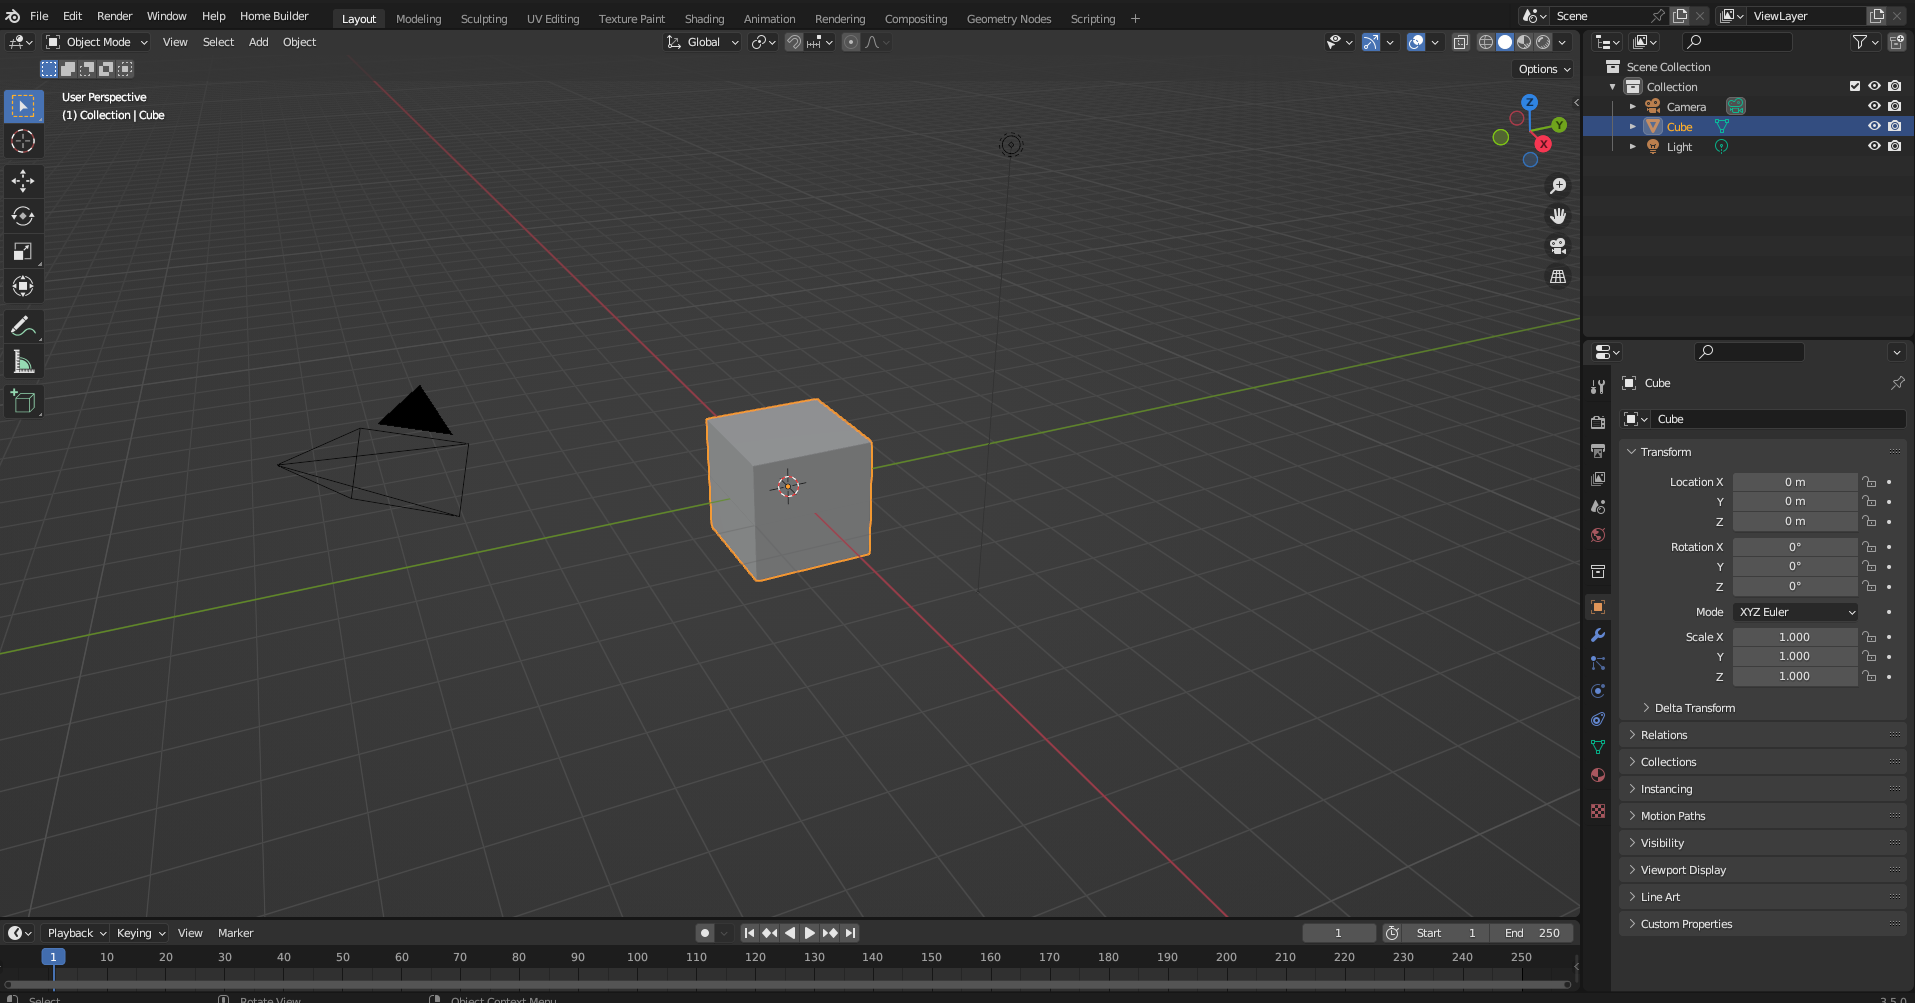
\includegraphics[width=0.8\textwidth]{chapters/13/images/3D-Viewport.png}
    \caption{In dieser Abbildung sind man den Objekt Mode von Blender.}
    \label{UST-8}
\end{figure}


\subsection{Edit Mode}
Dieser Modus bietet eine Reihe von Tools, um die gewünschte Form des Objekts zu erzeugen.
Diese Tools sind:


\begin{itemize}
    \item \textbf{Extrudieren}:
    \indent Das Extrudieren verwendet werden, um eine Fläche höher oder tiefer zu ziehen und somit als neuer Würfel zu dem Objekt hinzuzufügen.
    \begin{figure}[H]
        \centering
        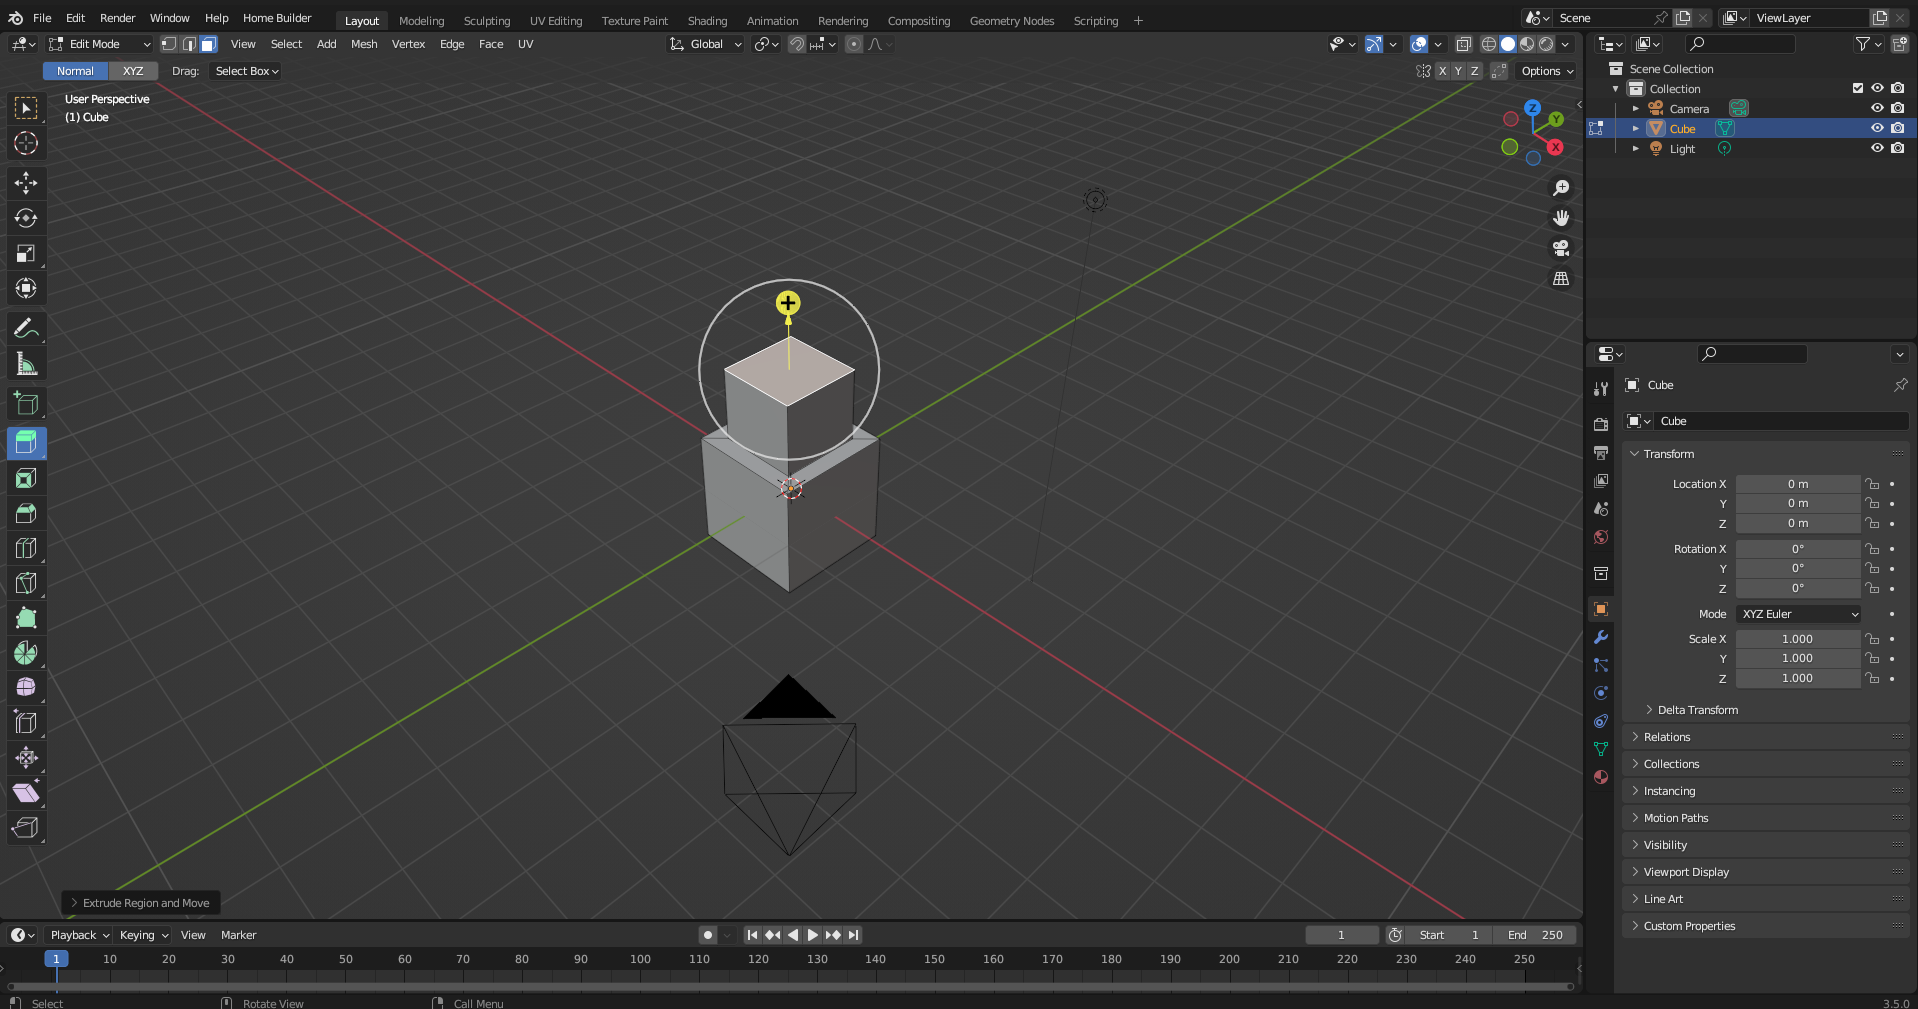
\includegraphics[width=0.8\textwidth]{chapters/13/images/ExtrudeTool.png}
        \caption{In dieser Abbildung sind man wie eine Fläche extrudiert wurde.}
        \label{UST-9}
    \end{figure}
    
    \item \textbf{Inset Faces}:
    \indent Das Inset Faces Tool ermöglicht das Erstellen von neuen Flächen innerhalb einer ausgewählten Fläche, was beispielsweise für die Erstellung von Löchern oder symmetrischen Auswuchtungen benötigt wird.
    \begin{figure}[H]
        \centering
        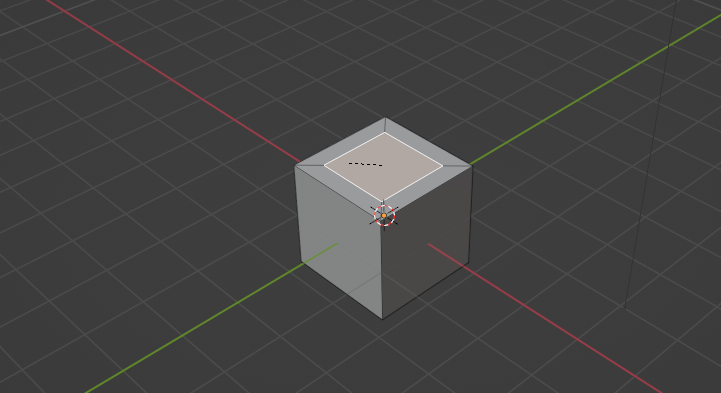
\includegraphics[width=0.8\textwidth]{chapters/13/images/InsetFace.png}
        \caption{In dieser Abbildung sind man eine Fläche in einer anderen Fläche erstellt.}
        \label{UST-10}
    \end{figure}
    
    \item \textbf{Loop Cut}:
    \indent Mit dem Loop Cut Tool können zusätzliche Kanten um das Objekt erstellt werden. Hiermit werden symmetrisch zum Objekt neue Kanten erstellt.
    \begin{figure}[H]
        \centering
        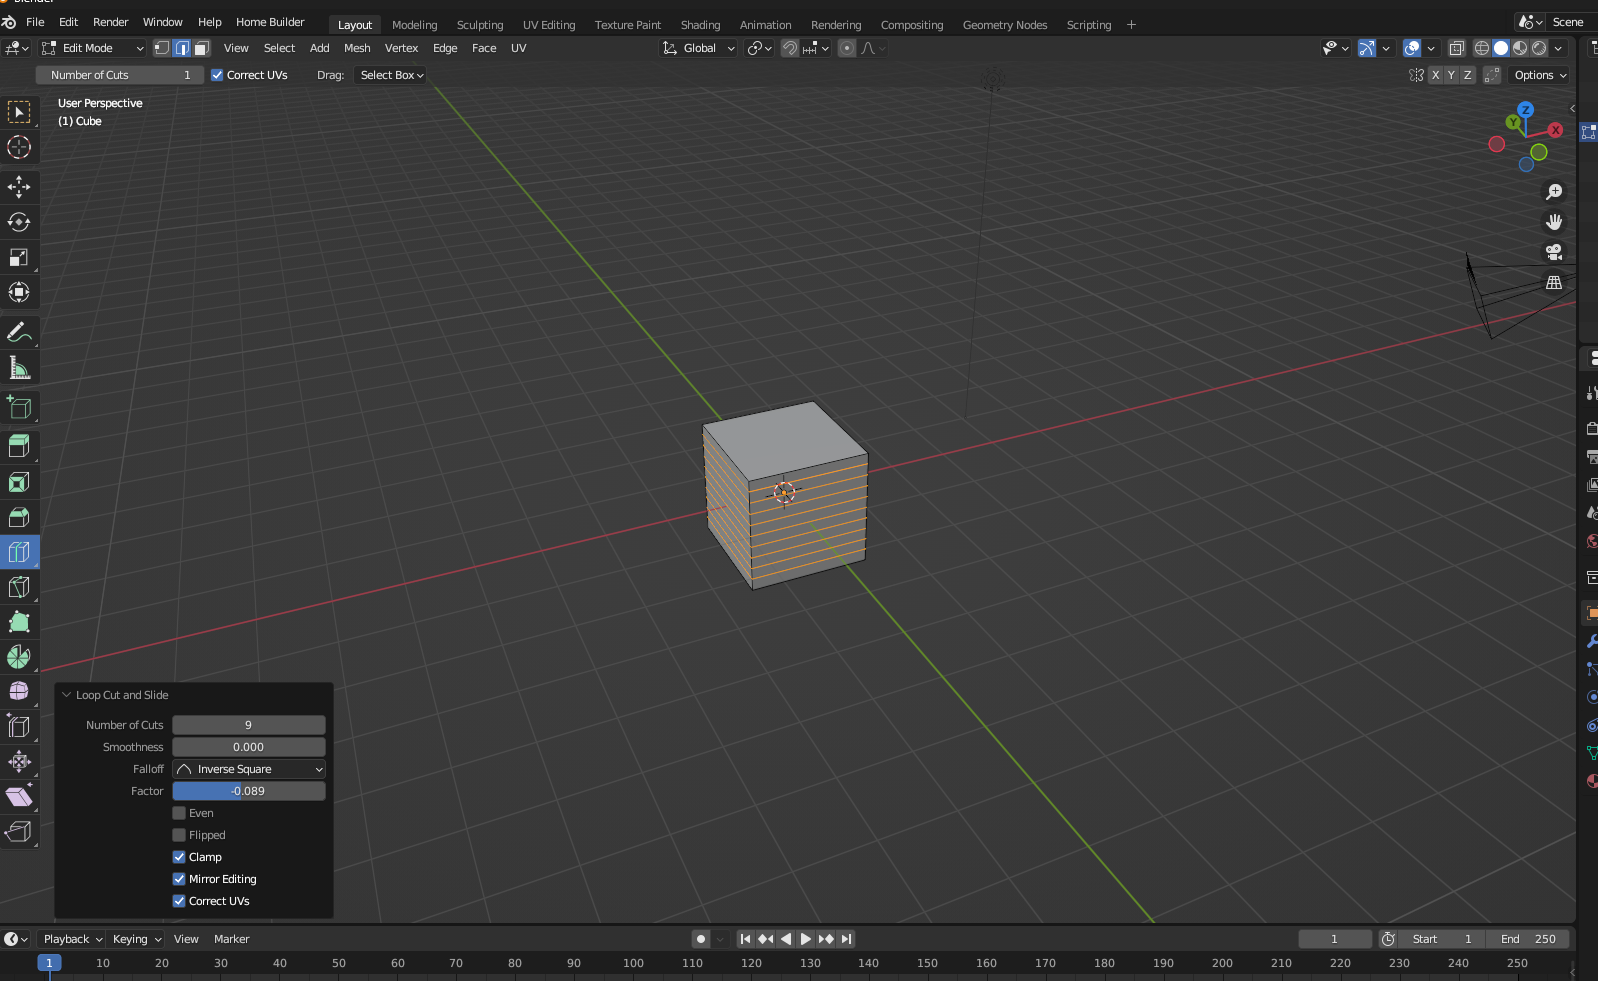
\includegraphics[width=0.8\textwidth]{chapters/13/images/Loopcut.png}
        \caption{In dieser Abbildung sieht man die Anwendung des Lopcut Tools.}
        \label{UST-11}
    \end{figure}
    \item \textbf{Messer}:
    \indent Das Messer Tool ermöglicht, Kanten mit der Freihand hinzuzufügen. Das wird benötigt, um Kanten an nicht symmetrischen Stellen zu erzeugen.
    \begin{figure}[H]
        \centering
        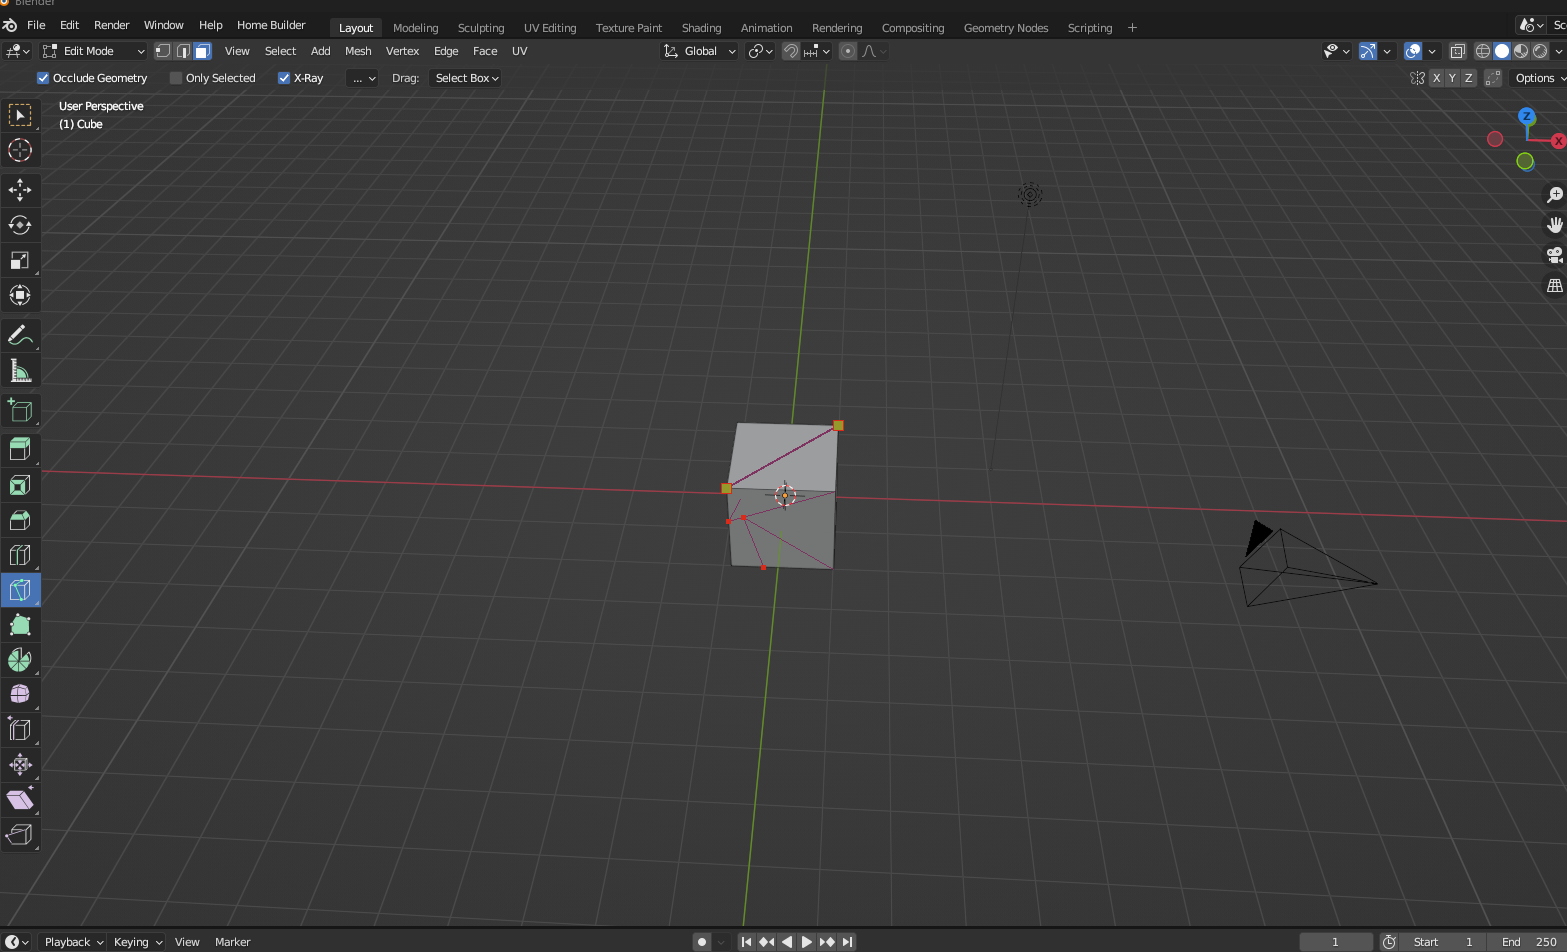
\includegraphics[width=0.8\textwidth]{chapters/13/images/KniveTool.png}
        \caption{In dieser Abbildung sieht man die Anwendung des Knive Tools.}
        \label{UST-12}
    \end{figure}
    \item \textbf{Poly Builder}: 
    \indent Schließlich bietet das Poly Builder Tool die Möglichkeit, einzelne Kanten zu markieren und die Länge zu verändern, um das Objekt nach Belieben zu verändern.
    \begin{figure}[H]
        \centering
        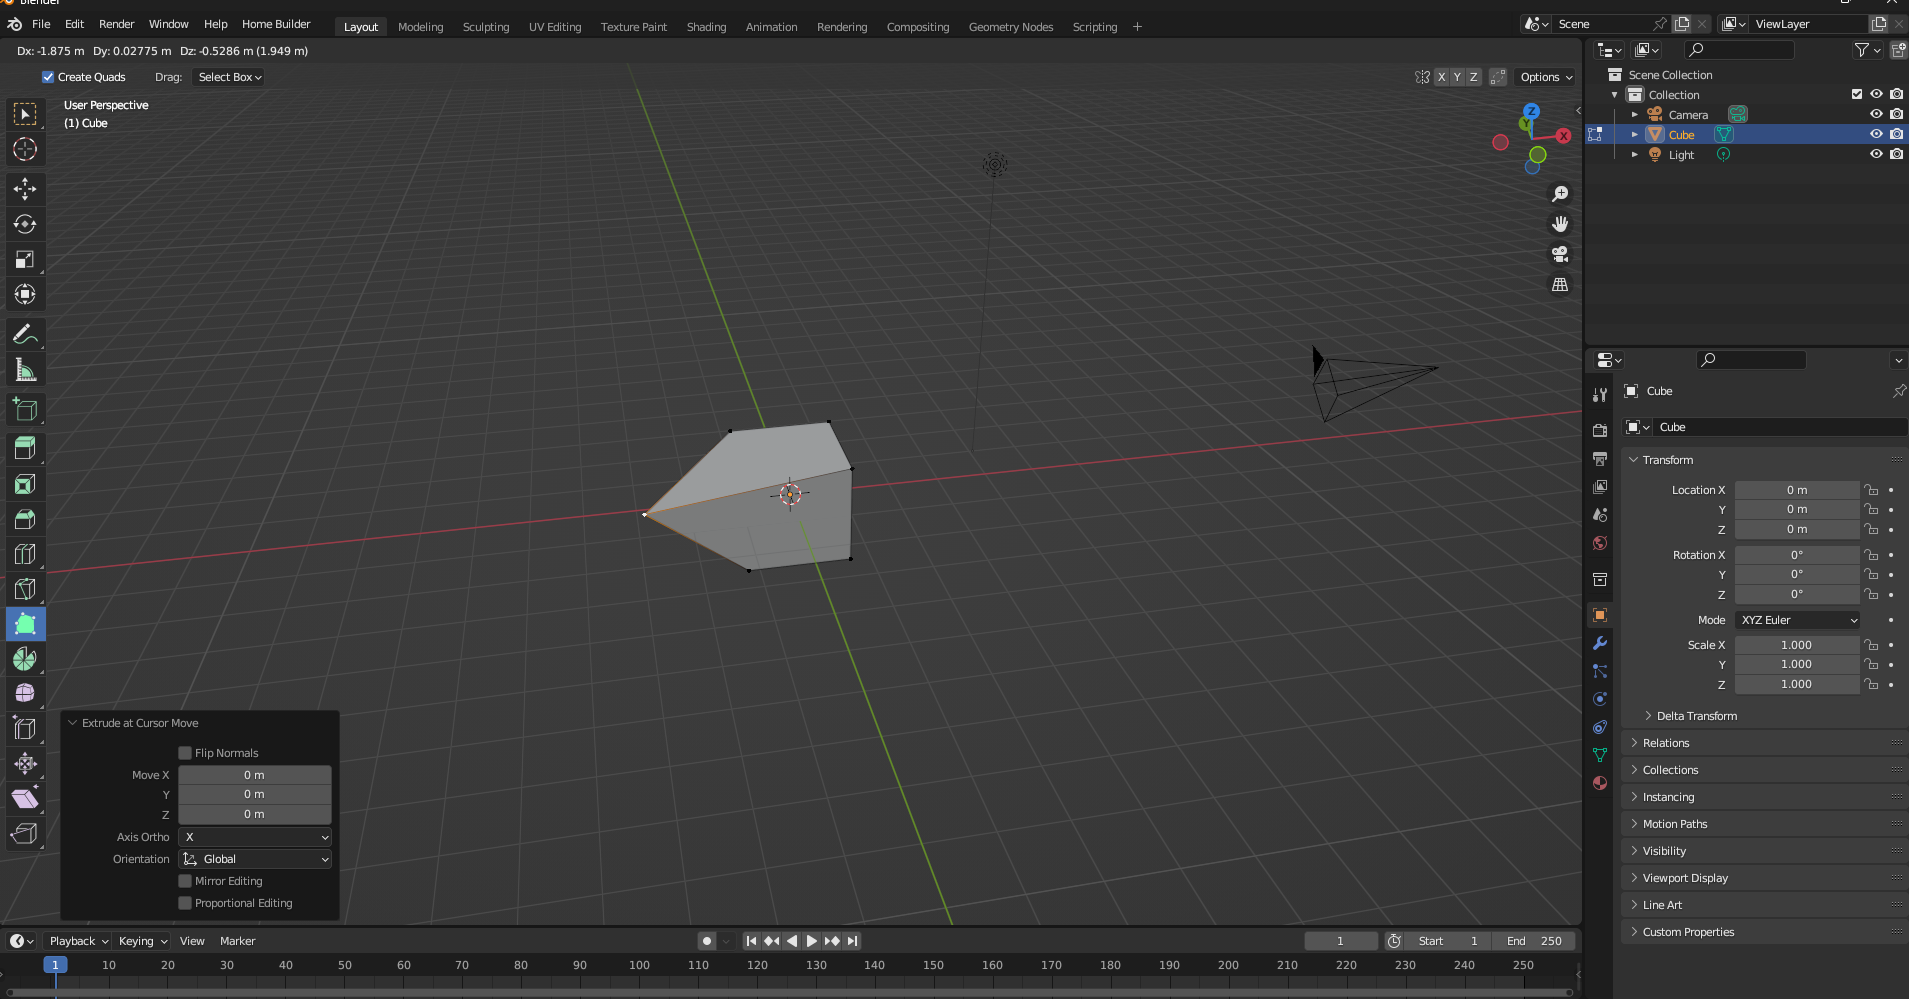
\includegraphics[width=0.8\textwidth]{chapters/13/images/PolyBuild.png}
        \caption{In dieser Abbildung sieht man die Anwendung des Poly Build Tools.}
        \label{UST-13}
    \end{figure}
\end{itemize}
%https://docs.blender.org/manual/en/latest/editors/3dview/modes.html

\subsection{Sculping Mode}
Der Sculping Mode hat verschiedene Tools um das Obejekt dynamisch zu verändern. In diesem Tool kann die \bettergls{topology}{1} bearbeitet werden. Hier kann die Anzahl der Polygone wie im Edit Mode dynamisch verändert werden. Die Arbeitsweise in diesem Tool ist wie folgt.\\\\
Zuerst werden grobe Details des Obejekt erzeugt wie Zum Beispiel die Grundform des Obejekt.\\\\
\begin{figure}[H]
    \centering
    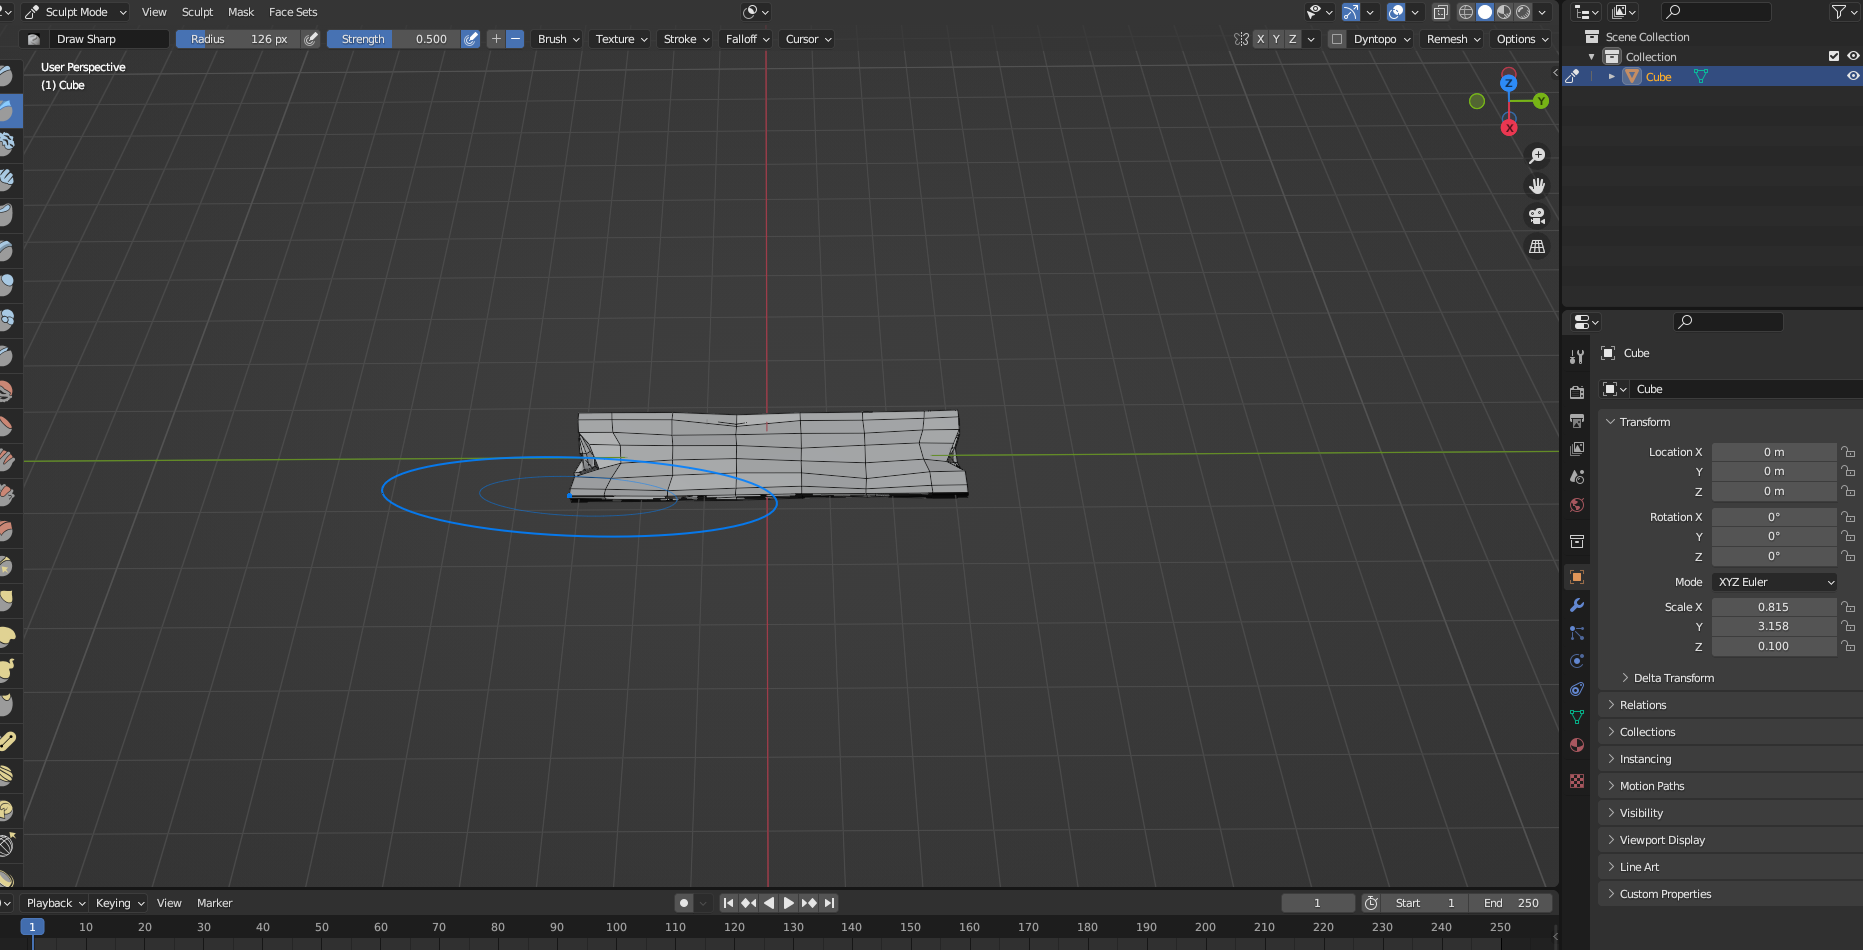
\includegraphics[width=0.8\textwidth]{chapters/13/images/HolzBrett.png}
    \caption{In dieser Abbildung zeigt die Bearbeitung der Grundform eines Spielobjekts.}
    \label{UST-14}
\end{figure}
\noindent Danach wird die Anzahl der Polygone erhöht um feinere Details hinzuzufügen. Dieser Workflow dient dazu so immer auf einer Detailstufe zu bleiben.
\begin{figure}[H]
    \centering
    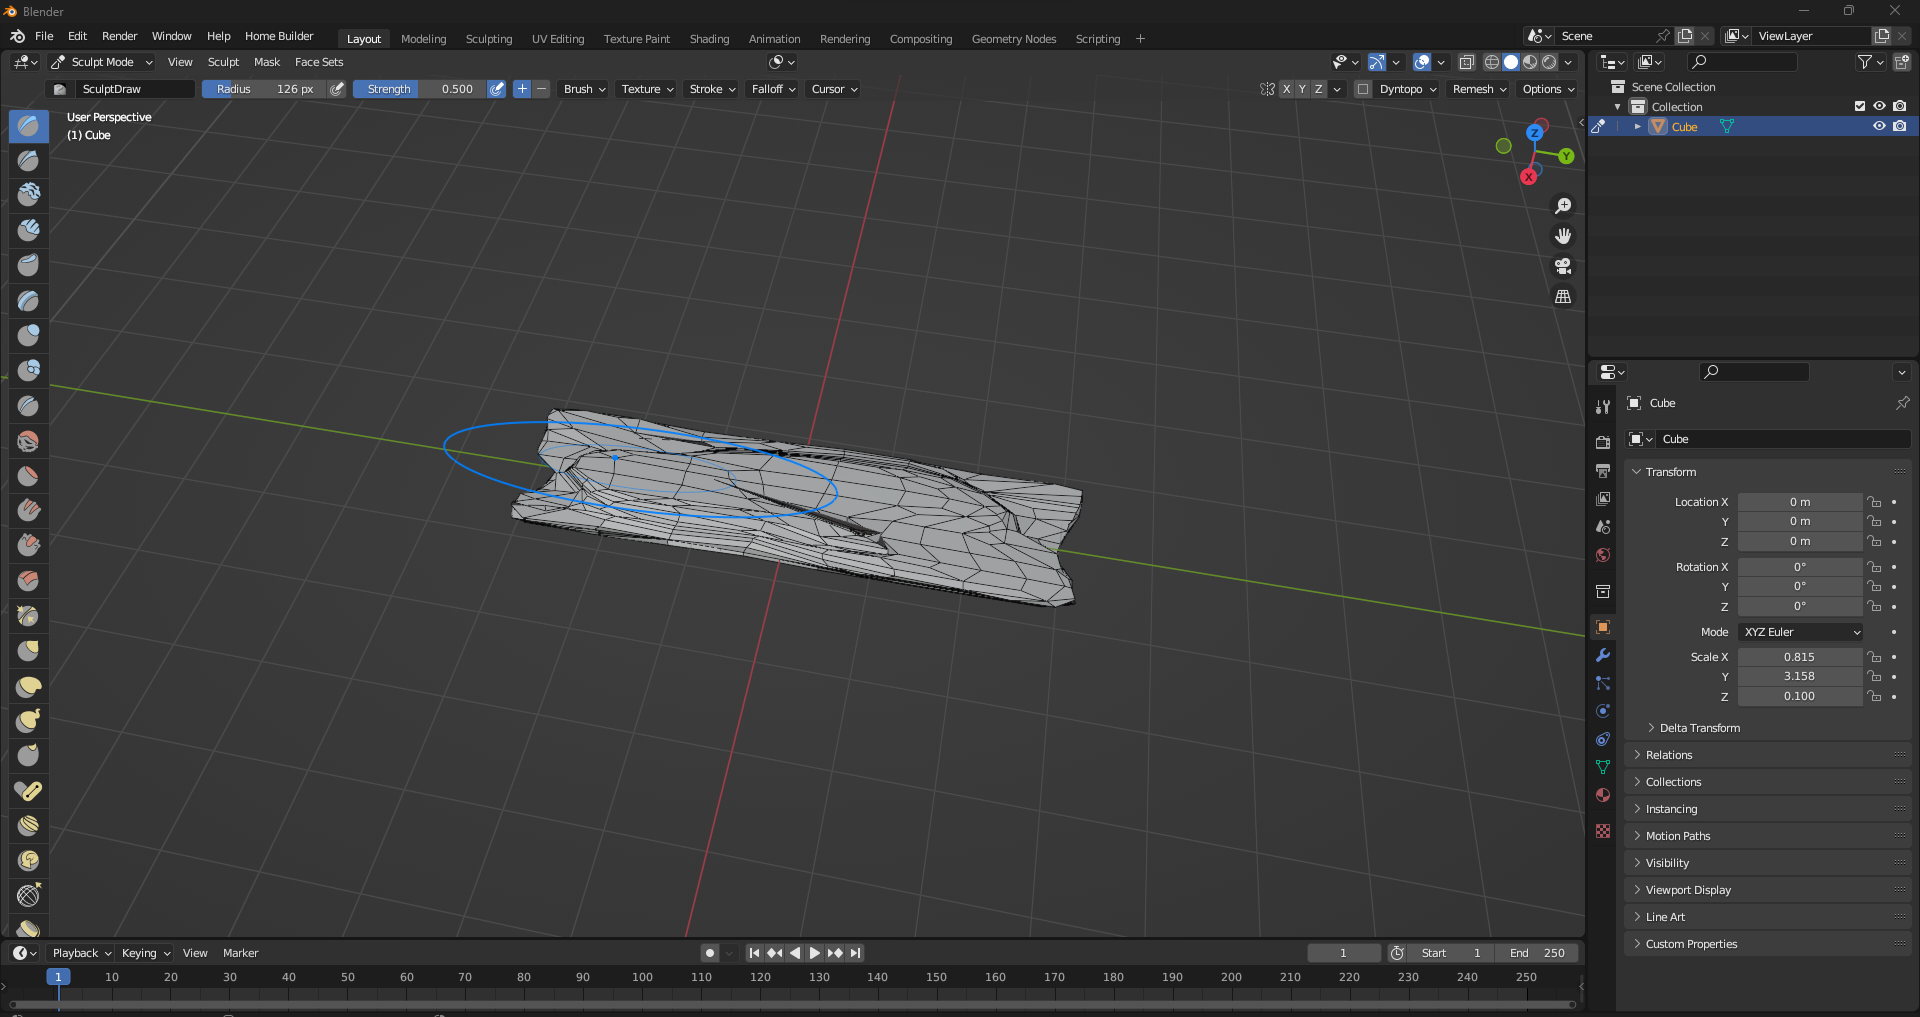
\includegraphics[width=0.8\textwidth]{chapters/13/images/HolzBrett1.png}
    \caption{In dieser Abbildung zeigt die Bearbeitung gröberer Details mit einer höheren Polygon anzahl.}
    \label{UST-15}
\end{figure}
\noindent Dieser Ablauf wird 2 bis 3 mal wiederholt um ein schönes detailiertes Objekt zu erstellen.
\begin{figure}[H]
    \centering
    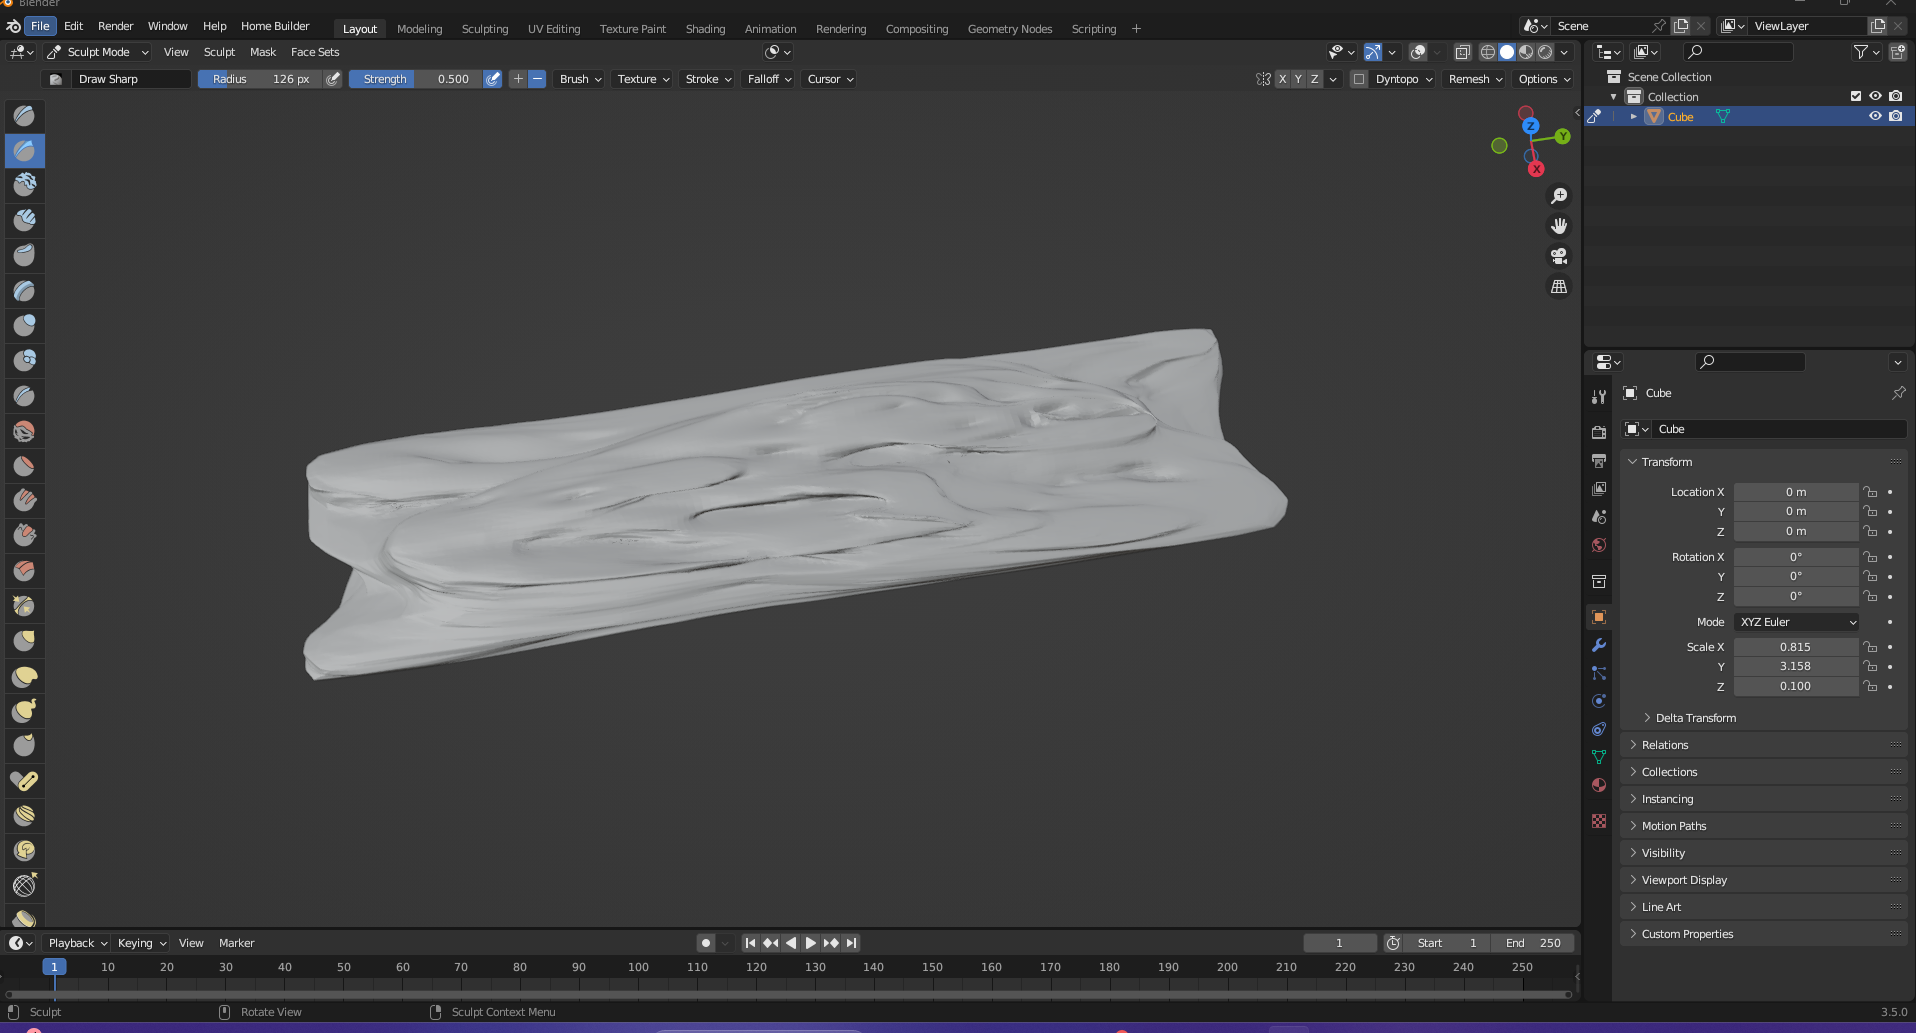
\includegraphics[width=0.8\textwidth]{chapters/13/images/HolzBrett2.png}
    \caption{In dieser Abbildung zeigt die Bearbeitung feinere Details auf das Objekt.}
    \label{UST-16}
\end{figure}
\noindent Wichtig ist darauf zu achten, dass je mehr Polygone das Objekt besitzt desto mehr muss berechnet werden. Das kann zum weiteren, zur schlechteren Performance im Spiel verusachen. Der letzte Schritt ist dann wieder das Runterskalieren der Objekte. Dieser ist Schritt ist wichtig um unnötige Polygone nicht zu laden. Wichtig dabei ist, dass die Details bebehalten werden. Um das zu gewehrleisten werden bestimmte Flächen wo keine Details exestieren runter Skaliert. in der Folgenden Abbildung kann man erkennen das in Orange die Fläche ist die keine Details besitzt und somit runterskaliert wurde.

\begin{figure}[H]
    \centering
    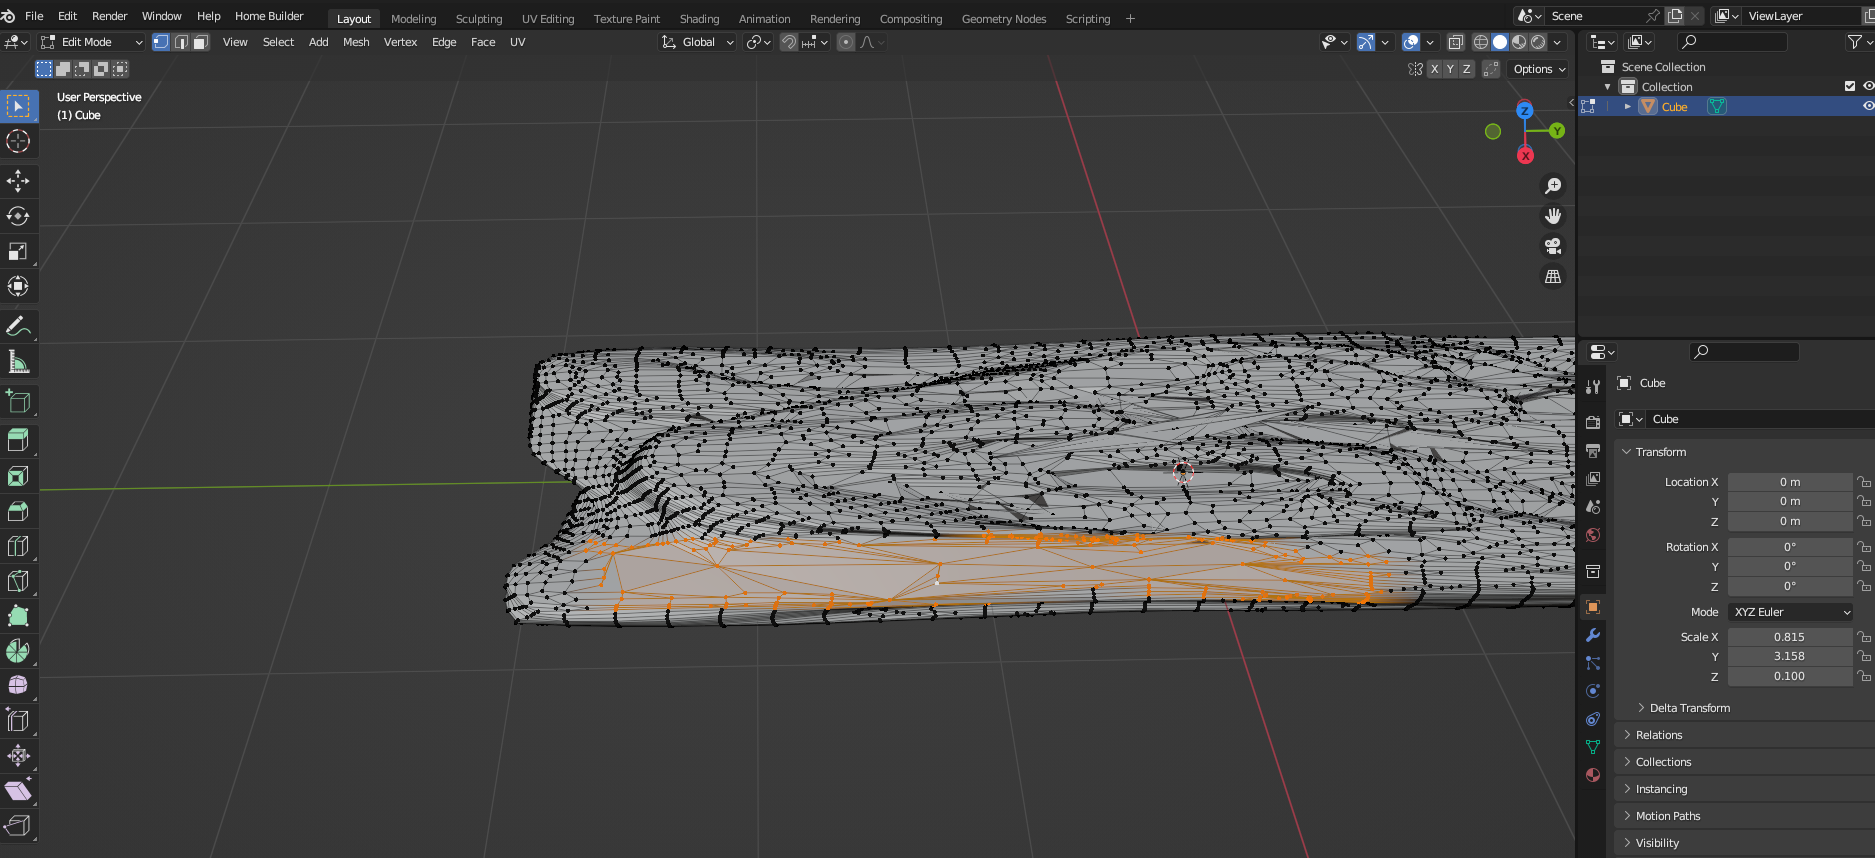
\includegraphics[width=0.8\textwidth]{chapters/13/images/HolzBrett3.png}
    \caption{In dieser Abbildung zeigt die runterskalierung einer Fläche auf dem Objekt.}
    \label{UST-17}
\end{figure}